\chapter{Loading data sets}
\label{ch:loading_data}

\newthought{The data sets we have worked with} in the previous lesson come with the \mutation\ installation. \mutation\ can read data from many file formats which include tab and comma separated and Excel files. To see how this works, let's prepare a data set (with school subjects and grades) in Excel and save it on a local disk.

\begin{figure}[h]
  \centering
  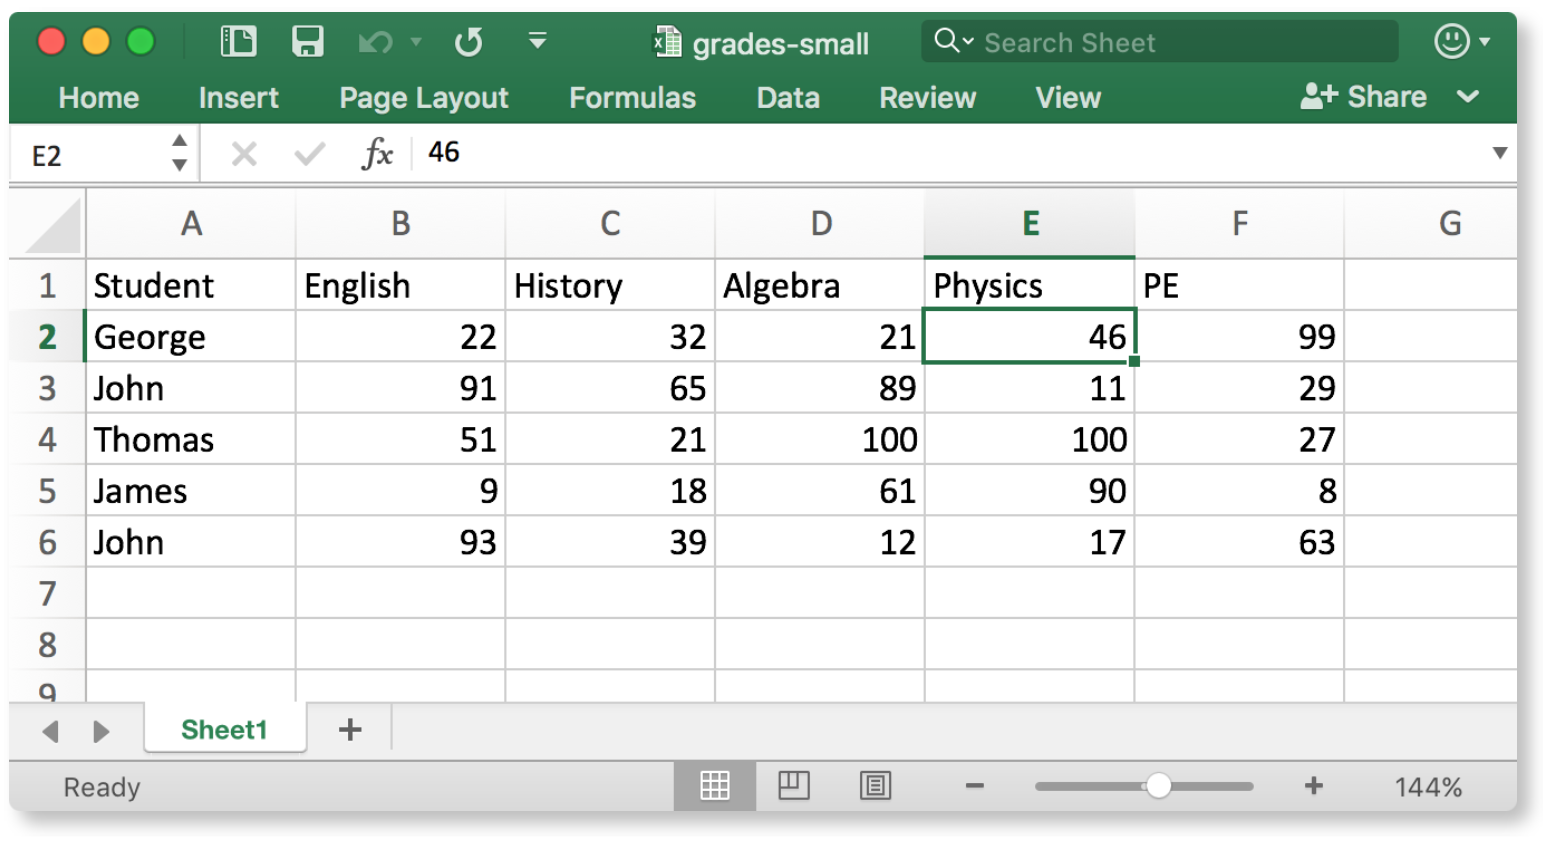
\includegraphics[width=\linewidth]{loading-fig1.png}%
  \caption{Make a spreadsheet in Excel with the numbers shown on the left. Of course, you can use any other editor, but remember to save your file in the \textit{comma separated values} (*.csv) format.}
  \label{fig:loading-fig1}
\end{figure}

In \mutation, we can use, for example, the File widget to load this data set.

\begin{figure}[h]
  \centering
  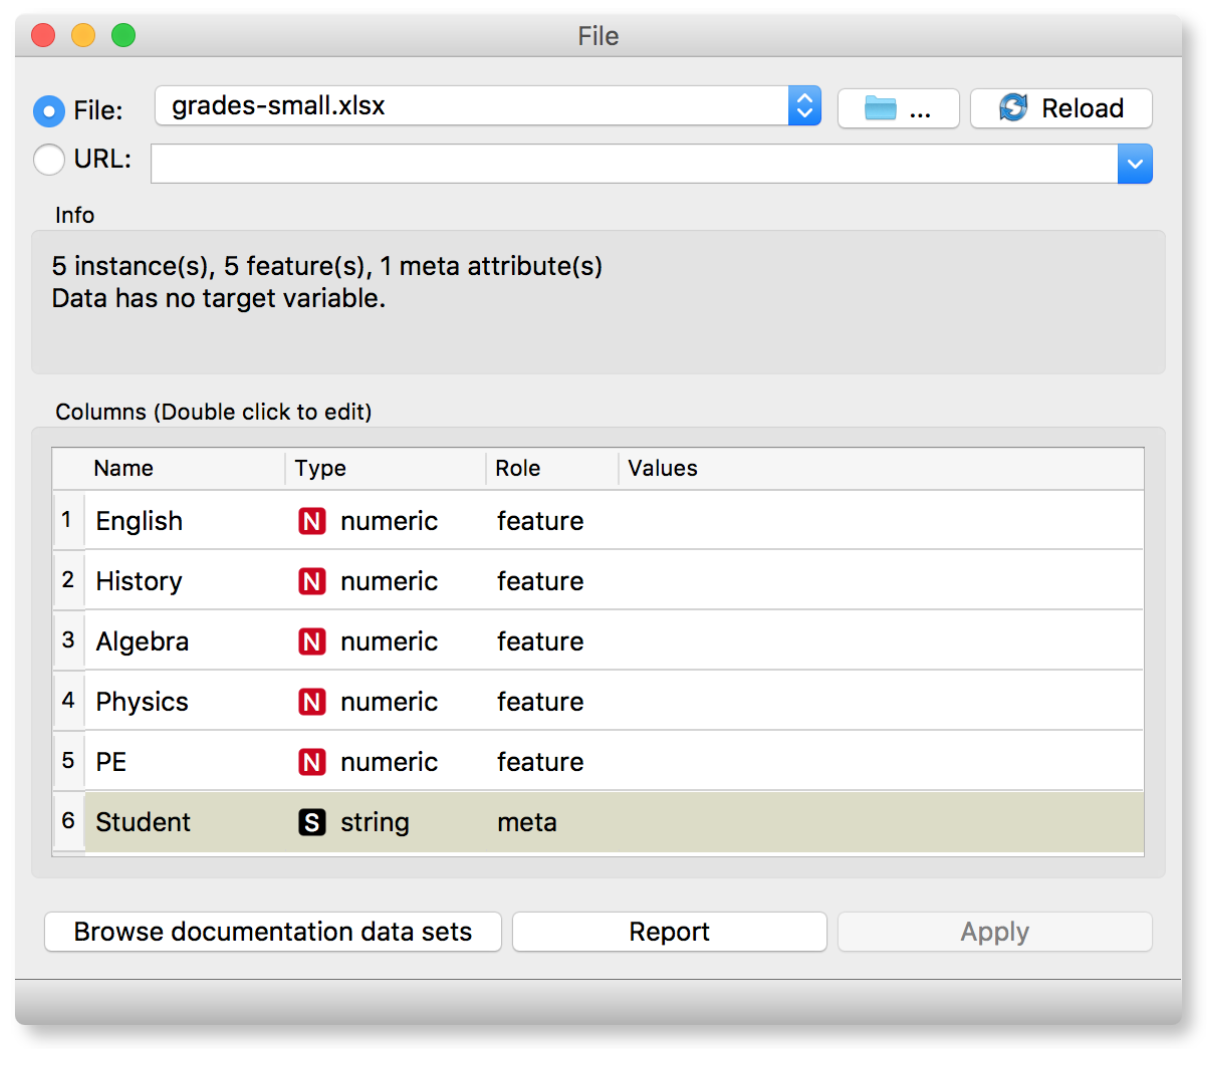
\includegraphics[width=90mm]{loading-fig2.png}%
  \caption{The \textit{File} widget allows you to select a local file or even paste a URL to a Google Spreadsheet. In the Info box, you will see a quick summary about the data you loaded. By double clicking the fields, you can also edit the types of entries and their role, that will be relevant for further processing.}
  \label{fig:loading-fig2}
\end{figure}

Looks good! \mutation\ has correctly guessed that student names are character strings and that this column in the data set is special, meant to provide additional information and not to be used for any kind of modeling (more about this in the upcoming lectures). All other columns are numeric features.

It is always good to check if all the data was read correctly. Now, you can connect the \textit{File} widget with the \textit{Data Table} widget,

\begin{figure}[h]
  \centering
  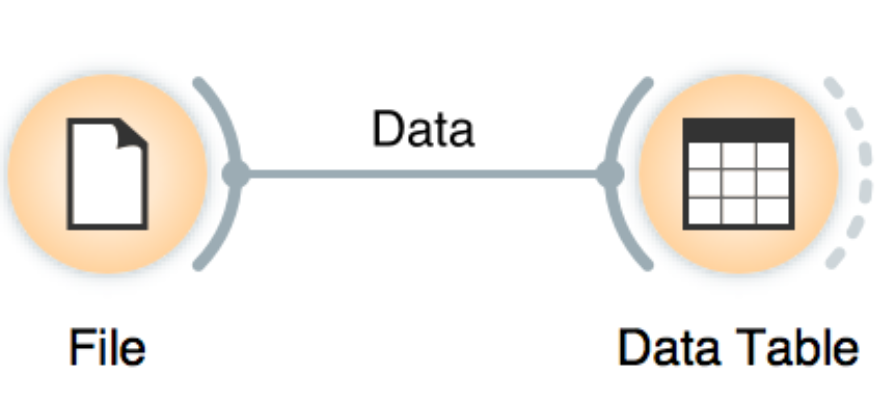
\includegraphics[width=40mm]{loading-fig3.png}%
  \caption{Make the simple workflow shown on the right.}
\label{fig:loading-fig3}
\end{figure}

\noindent and double click on the Data Table to see the data in a spreadsheet format.
Nice, everything is here. 

\begin{figure*}[h]
  \centering
  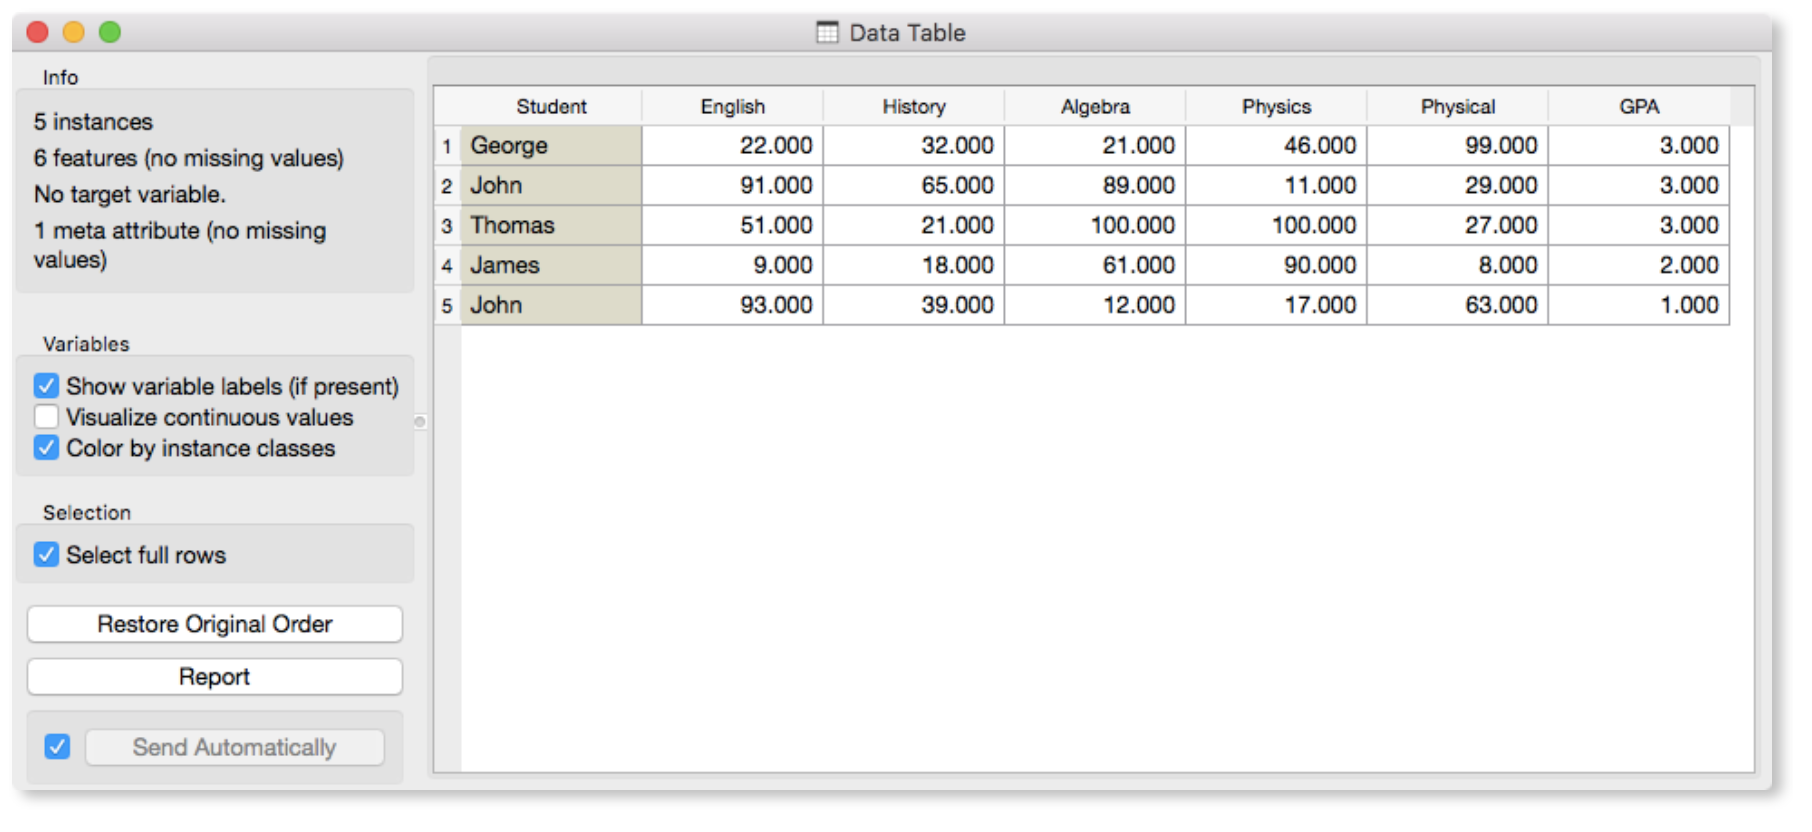
\includegraphics[width=\linewidth]{loading-fig4.png}%
  \caption{The \textit{Data Table} widget shows the loaded data set, you can select rows, which will appear on the output of the widget. It is also possible to do simple data visualizations. Explore the functionalities!}
  \label{fig:loading-fig4}
\end{figure*}

Instead of using Excel, we could also use Google Sheets, a free on-line spreadsheet alternative. Then, instead of finding the file on the local disk, we would enter its URL address to the File widget URL entry box.

\mutation’s legacy native data format is a tab-delimited text file with three header rows. The first row lists the attribute names, the second row defines their type (continuous, discrete, time and string, or abbreviated c, d, t, and s), and the third row an optional role (class, meta, weight, or ignore).

There is more to input data formatting and loading. If you would really like to dive in for more, check out the documentation page on \href{https://orange-visual-programming.readthedocs.io/loading-your-data/index.html}{Loading your Data}, or a \href{https://www.youtube.com/watch?v=MHcGdQeYCMg}{video tutorial} on this subject.
